\section{Results}\label{sec:Results}
To find the optimal parameters for our machine learning methods, we performed a cross-validation grid search. The results are presented in table \ref{tab:configuration}. For the three boosting methods the following ranges were tested for each parameter:

\begin{itemize}
    \item Estimators: 100, 150, 200.
    \item Max depth: 5, 7, 9, 11.
    \item Learning rate: 1, 0.5, 0.1.
\end{itemize}

For the bagging and random forest methods we did a search over the following parameter space:

\begin{itemize}
    \item Estimators: 100, 150, 200, 250, 300.
    \item Max depth: 3, 5, 7, 9, 11, 13, 15.
\end{itemize}

In the case of the simple decision tree, we did a tree depth search from $2$ to $20$. We have also used both the gini index and information entropy as node impurity measures for the trees, in which the information entropy gave the best scores in every case. 

Figure \ref{fig:simple_tree_crossval} shows the validation curve of the simple decision tree, in which we found that a depth of $19$ was optimal, giving an accuracy score of $97.8$ on the test data. We see from the figure that a tree with only depth $2$ has roughly a $50\%$ accuracy of predicting the correct class among the $7$, with an increasing trend until it reaches a tree depth of approximately 13, after which both the validation and training scores remain constant.

\begin{figure}
    \centering
    \includegraphics[scale=0.6]{Figures/20191205-131043_simple_tree_tree_depth_opt.pdf}
    \caption{Validation curve of a simple decision tree on the setting 1 data. Optimal tree depth is 19, with validation score 97.5 and test score 97.8.}
    \label{fig:simple_tree_crossval}
\end{figure}

Table \ref{tab:accuracy} shows the accuracy of our ensemble methods, with their optimal parameter configurations listed in table \ref{tab:configuration}. We see that gradient boosting and XGBoost have the best performance with an accuracy score of $99.5$, while AdaBoost and random forests perform almost equally as well with accuracy scores of $99.1$. The bagging classifier is only slightly worse with a score of $97.8$. Using setting 2, gradient boosting performs best with a score of $19.5$, while the rest of the classifiers are below $14$. 

In table \ref{tab:ravi_results} we present the results from a similar research paper on human activity recognition from Ravi et al.\cite{ravi}. This paper compared several machine learning methods, and we have included the ones that matches the methods of our project. Ravi et al. used raw data from a triaxial accelerometer, akin to us, and extracted a similar feature set to ours, by using window sampling to calculate mean, standard deviation etc. The sampling window was however $5.12$ seconds, while ours was $1$ second, and they extracted some additional features (details can be found in the original research paper\cite{ravi}). Also note that setting 2 is defined slightly different in this case, as mentioned in the table caption. For setting 1, the decision tree outperformed bagging and boosting with a score of $98.53$, while bagging gave the best performance in setting 2, with a score of $63.33$.

Figure \ref{fig:confusion_matrix} shows the confusion matrices for the best performing classifiers in both setting 1 and 2. The feature importances are shown in figure \ref{fig:feature_importance}, estimated for all the methods we tested in this project. The overall best performing classifier, gradient boosting, is highlighted in red. Feature 4, standard deviation of $y$-acceleration, stands out as the most significant feature in most methods, while 5-8 (standard deviation of $z$-acceleration and ranges of all axes) are generally regarded as relatively unimportant.

\begin{table}[]
\caption{Configuration of the classifiers for the two different cases, found by performing a cross-validation grid search on the parameters.}
\begin{tabular}{|l|c|c|c|c|c|c|}
\hline
\multirow{2}{*}{Classifier} & \multicolumn{3}{c|}{Setting 1}            & \multicolumn{3}{c|}{Setting 2}            \\ \cline{2-7} 
                            & Estimators & Max depth & Learning rate & Estimators & Max depth & Learning rate \\ \hline
Decision tree               & 1          & 19        & N/A           & 1          &17         & N/A           \\ \hline
Bagging                     & 200        & 15        & N/A           &  200       & 15        & N/A           \\ \hline
Random forest               & 200        & 15        & N/A           &  300       & 15        & N/A           \\ \hline
AdaBoost                    & 150        &  11      & 1             &  200       &  11     &  1             \\ \hline
Gradient boosting           & 200       & 7          & 0.1             & 200       & 7    &  0.1             \\ \hline
XGBoost                     &  200      &  5        &  0.5          &  200         &  7         &   0.5            \\ \hline
\end{tabular}'
\label{tab:configuration}
\end{table}

\begin{table}[]
\caption{Accuracy of classifiers for the two different settings.}
\begin{tabular}{|l|c|c|}
\hline
\multirow{2}{*}{Classifier} & \multicolumn{2}{c|}{Accuracy (\%)} \\ \cline{2-3} 
                            & Setting 1           & Setting  2          \\ \hline
Decision tree               & 97.8             & 7.2             \\ \hline
Bagging                     & 98.9             & 12.0            \\ \hline
Random forest               & 99.1             & 10.9            \\ \hline
AdaBoost                    & 99.1             & 13.5            \\ \hline
Gradient boosting           & 99.5             & 19.5            \\ \hline
XGBoost                     & 99.5             & 13.6             \\ \hline
\end{tabular}
\label{tab:accuracy}
\end{table}


\begin{table}[]
    \centering
    \caption{Results from the research paper by Ravi et al.\cite{ravi}. Note that in this case setting 2 consisted only of data from one subject, while the test data was from another subject (setting 1 and 2 corresponds to respectively setting 2 and 4 in the paper by Ravi et al.).}
    \begin{tabular}{|l|c|c|}
\hline
\multirow{2}{*}{Classifier} & \multicolumn{2}{c|}{Accuracy (\%)} \\ \cline{2-3} 
                            & Setting 1         & Setting  2        \\ \hline
Decision tree               & 98.53             & 57.00             \\ \hline
Bagging                     & 95.22             & 63.33            \\ \hline
Boosting                    & 98.35             & 57.00     \\ 
\hline
\end{tabular}
    \label{tab:ravi_results}
\end{table}


\begin{figure}
    \centering
    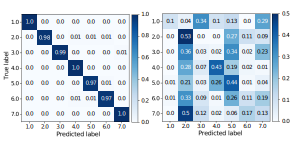
\includegraphics[scale=0.48]{Figures/confusionmatrix_double.pdf}
    \caption{Confusion matrices. Left: Setting 1, using XGBoost. Right: Setting 2, using gradient boosting.}
    \label{fig:confusion_matrix}
\end{figure}

\begin{figure}
    \centering
    \includegraphics[scale=0.7]{Figures/featimp-case1.pdf}
    \caption{Feature importance. The feature indeces are found in table \ref{tab:features}.}
    \label{fig:feature_importance}
\end{figure}


 